In an attempt to create a model based controller that can be applied to the soft robotic actuator, the developed non-linear model should first be validated. This is done by using a planar 2 degree-of-freedom soft robot. This robot has a translational and rotational degree of freedom. Rotation is only dependent on the difference in bellow length, not absolute bellow length. To measure rotation, an Inertial Measurement Unit (IMU) is connected at the tip of the robot. The position of the bellows can be tracked with a camera set-up. From this data, elongation and curvature of each individual bellow can extracted. Being able to measure/determine both degrees-of-freedom allows us to validate the dynamic model. 

\section{Model validation for the planar soft actuator}


\subsection{Measuring Devices}




\subsection{Forward kinematics of the planar robot}

To describe the configuration space of the soft robot, it is regarded as a continuous deformable structure with infinite degrees of freedom.
A model that describes the configuration space of the soft robotic manipulator as a function of space and time was formulated in \cite{Caasenbrood2020}. The model is based on a one-dimensional Cosserat beam together with geometrically exact beam theories proposed in \cite{Simo1986}.

Consider a spatial coordinate $\sigma \in \mathbb{X}$ within the bounded domain $\mathbb{X} \in [0,l] \subset \mathbb{R}$, and a temporal coordinate $t \in  \mathbb{T}$ with $\mathbb{T} \subseteq \mathbb{R}$. Given these notations, position $p(\sigma,t) \in \mathbb{R}^3$ and rotation matrix $R(\sigma,t) \in \mathbb{SO}(3)$ can be given for any point $\sigma$ and instance $t$ on the continuous backbone of the soft manipulator by,

\begin{equation}
    g(\sigma,t) := \begin{pmatrix}  R(\sigma,t) & p(\sigma,t) \\ 0_3^\top & 1 \end{pmatrix} \in \mathbb{SE}(3)
    \label{eq2:g}
\end{equation}

where $\mathbb{SE}(3)$ is the Lie group of rigid body transformations in $\mathbb{R}^3$ \cite{Sola2018}. Since function $g$ is space and time variant, changes in space and time can be captured by two vector fields in the Lie algebra $\mathfrak{se}(3)$. Partial derivatives $\partial (.)/\partial(\sigma)$ and $\partial (.)/\partial(t)$ will be denoted by a `prime' and `dot' for position and time, respectively. The partial derivative with respect to time of (\ref{eq2:g}) results in the time-twist field described by,


\begin{equation}
    \frac{\partial g}{\partial t} = \dot{g} = g\hat{\eta} \Longrightarrow \hat{\eta} := g^{-1}\dot{g} = \begin{pmatrix} \Omega_\times & V \\ 0_3^\top & 0 \end{pmatrix} \in  \mathfrak{se}(3)
    \label{eq2:dotg}
\end{equation}

where $\Omega = (\omega_1,\omega_2,\omega_3)^\top$ and $V = (v_1,v_2,v_3)^\top$ express vectors of angular velocity and linear velocity, respectively. The skew-symmetric matrix $\Omega_\times$ can be related to $\mathfrak{so}(2) \cong \mathbb{R}^3$ given the mapping $\Omega \mapsto \Omega_\times$ \cite{Sola2018}. Here, vector field $\eta(\sigma,t)$ describes an infinitesimal local transformation by a frame at position $\sigma$ between infinitesimally small $t$ and $t+\Delta t$. Following the same logic, the partial derivative of (\ref{eq2:g}) with respect to space results in the space-twist field defined as,


\begin{equation}
   \frac{\partial g}{\partial \sigma} =  g' = g\hat{\xi} \Longrightarrow \hat{\xi} := g^{-1}g' = \begin{pmatrix} K_\times & E \\ 0_3^\top & 0 \end{pmatrix} \in  \mathfrak{se}(3)
    \label{eq2:gaccent}
\end{equation}

in which $K = (k_1,k_2,k_3)^\top$ and $E = (\epsilon_1,\epsilon_2,\epsilon_3)^\top$ represent vectors containing the curvature-torsion strain and stretch-shear strain, respectively. Likewise, vector field $\xi(\sigma,t)$ describes an infinitesimal local transformation by a frame at time instance $t$ between infinitesimally small $\sigma$ and $\sigma+\Delta \sigma$. Because $\mathfrak{se}(3) \cong \mathbb{R}^6$ and with mapping $\eta \mapsto \hat{\eta}$, (\ref{eq2:dotg}) and (\ref{eq2:gaccent}) can be formulated as a column vector in $\mathbb{R}^6$ as


\begin{equation}
    \eta(\sigma,t) = \begin{pmatrix} \Omega \\ V \end{pmatrix}; \hspace{20pt} \xi(\sigma,t) = \begin{pmatrix} K \\ E \end{pmatrix}
    \label{eq2:etaxi}
\end{equation}

For solving the forward kinematics only position of the soft robotic manipulator is of interest, hence the following first order partial differential equation (PDE) needs to be solved for spatial coordinate $\sigma$ only,

\begin{equation}
    \frac{\partial g}{\partial \sigma} = g \hat{\xi}
    \label{eq2:dgdsigma}
\end{equation}

To solve this PDE, it is transformed to an ordinary differential equation (ODE) which is suitable for controller design. This is done by projecting the infinite-dimensional system onto a subspace of finite dimension which contains basis elements of the expected solution. By reducing the dimensionality of the system, higher order dynamics are not captured in the model, therefore robustness should be taken into account. To transform PDE (\ref{eq2:dgdsigma}), the components of the strain field $\xi := (g^{-1}g')$ are approximated using a finite amount of orthogonal shape functions, as follows

\begin{equation}
    \xi_i(\sigma,t) \cong \sum_{i=1}^N \varphi_i(\sigma)q_i(t) + \xi_{i,0}(\sigma), \hspace{20pt} \forall \sigma \in \mathbb{X}, t \in \mathbb{T}
\end{equation}

in which, $\xi_{i,0}$ corresponds to the undeformed configuration of the robotic manipulator, $\mathbb{X}$ a spatial set, and time set $\mathbb{T} \subseteq \mathbb{R}$. Additionally, $\{\varphi_i\}_{i \in \mathbb{N}}$ is a set of basis shape functions and $q(t)$ are modal coefficients. These modal coefficients can be thought of as generalized coordinates of the finite-dimensional system. The $n$-th order strain expansion can be formulated as

%% maybe write about what shape functions were used

\begin{equation}
\begin{aligned}
    \xi(\sigma,t) \cong & \hspace{5pt}  (B_a \otimes [ \varphi_1 \dots \varphi_N ])q(t)\\ = &  \underbrace{ \begin{pmatrix}
    \varphi_1(\sigma) & \dots  & \varphi_N(\sigma) & \dots     & 0      & \dots  &  0 \\
    \vdots    & \ddots & \vdots    & \ddots    & \vdots & \ddots & \vdots \\
    0         & \dots  & 0         & \dots     & \varphi_1(\sigma) & \dots & \varphi_N (\sigma)
    \end{pmatrix}}_{\Phi(\sigma)} \begin{pmatrix} q_1(t) \\ \vdots \\ q_n(t) \end{pmatrix} +  \begin{pmatrix} \xi_{1,0} \\ \vdots \\ \xi_{n,0}   \end{pmatrix}
    \end{aligned}
\label{eq2:xishape}
\end{equation}

where $\Phi : \mathbb{R} \mapsto \mathbb{R}^{m \times n}$ is a shape function matrix in which $n$ is equal to the amount of modal coordinates, and $m$ the amount of active strains, and $B_a \subseteq \text{span}(\mathbb{I}_6)$ a selection matrix of unconstrained strains. Within matrix $B_a$ the active strains are given a `1' and constrained stains `0'. For the planar soft robot one curvature-torsion strain and one stretch-shear strain are active. 


In Matlab \cite{MATLAB2020} a code was created to calculate the forward kinematics given modal coordinates $q(t)$. To reduce computation time of solving the ODE with \verb+ode45+, the 4 by 4 matrix $g(\sigma,t)$, Equation (\ref{eq2:g}), is rewritten as a column vector of size 7. To this end, the rotation matrix $R(\sigma,t)$ is rewritten to quaternion formulation as follows \cite{Boyer2019},


\begin{equation}
\frac{\partial}{\partial \sigma}    \begin{pmatrix} Q \\ p \end{pmatrix} = \begin{pmatrix} 2 ||Q||^{-1} A(R(Q)K)Q \\ R(Q)p \end{pmatrix}
\label{eq2:Qp}
\end{equation}

where $Q$ is the quaternion representation of rotation matrix $R$, and $R(Q)$ a function mapping a quaternion to rotation matrix representation, $A$ is a function defined as,


\begin{equation}
    A(K) = \begin{pmatrix} 0 & -K_1 & -K_2 & -K_3 \\ K_1 & 0 & -K_3 & \hspace{8pt}K_2 \\ K_2 & \hspace{8pt}K_3 & 0 & -K_1 \\ K_3 & -K_2 & \hspace{8pt}K_1 & 0 \end{pmatrix}
    \label{eq2:AK}
\end{equation}

where $K_i$ correspond to the entries of $xi(\sigma,t)$ shown in Equation (\ref{eq2:etaxi}). In Equation \ref{eq2:Qp} and \ref{eq2:AK} the dependency of $\sigma$ and $t$ has been omitted for the sake of readability.

\subsection{Inverse kinematics of the planar robot}

The developed forward kinematic model can be used for determining the inverse kinematics of the planar robot. This is done by a Jacobian search method. In essence, a desired position and orientation of the robot's end-effector is given. A Newton-Euler based optimization is carried out to find the modal coordinates $q(t)$ mapping to end-effector position $x,z,\theta$. This Newton-Euler search method uses the Jacobian which is given by \cite{Caasenbrood2020},

\begin{equation}
\eta(\sigma,t) = Ad_{g^{-1}(\sigma = l)} \int_{0}^{\sigma} Ad_g B_a \Phi(\sigma) d\sigma \dot{q} := J\dot{q}
\end{equation}

where $J(\sigma,q) \in \mathbb{R}^{6 \times n}$ is the jacobian matrix mapping modal velocities to the time-twist field, and $Ad_g$ is defined as the adjoint mapping found by,


\begin{equation}
    Ad_g = \begin{pmatrix} R & 0 \\ \hat{r}R & R \end{pmatrix}
\end{equation}

in which, $R$ is the rotation matrix at space instant $\sigma$, and $\hat{r}$ a 3x3 skew-symmetric matrix for which holds that $\hat{r}V = r \times V$ for any $V \in \mathbb{R}^3$ \cite{Boyer2019}.

\begin{equation}
    J^\dagger = wJ^\top(JwJ^top + \rho I_{6\times 6})^{-1}
\end{equation}


\begin{equation}
    q_{k+1} = q_{k} + \alpha J^\dagger (x_d - x_k)
\end{equation}
























\section{Stiffness Determination in FEM}








\subsection{Influence of (non)-linear material parameters}


The influence of linear/non-linear material parameters were investigated by pressurizing both bellows equally for 20kPa and 80kPa for both linear and non-linear material parameters. For the linear case a Young's modulus ($E$) of 69 Mpa and a Poisson ratio ($\nu$) of 0.45 were used. These parameters can be used to calculate the Lamé parameters necessary to simulate non-linear Neo-Hookeon deformation. To this end, Lamé's first parameter or shear modulus $\mu$ and bulk modulus $\kappa$ need to be calculated, these can be calculated with the following equations, respectively

\begin{equation}
    \mu = \frac{E}{2(1+\nu)}
\end{equation}


\begin{equation}
    \kappa = \frac{E}{3(1-2\nu)}
\end{equation}

In the Abaqus FEM environment these constants need to be translated to \verb+C10+ and \verb+D1+ parameters by the with

\begin{equation}
    \verb+C10+ = \frac{\mu}{2}
\end{equation}


\begin{equation}
    \verb+D1+ = \frac{2}{\kappa}
\end{equation}

As mentioned, two simulations were carried out pressurizing both bellows equally for 20kPa and 80kPa.Deformations in $x,y,z$ direction for both material parameters are shown in Table (\ref{tab2:linnonlindef}). The procedure to calculate deformation works as follows. After the bellows are pressurized, the nodes in the top plate are isolated. Hereby, we assume that the connection plate at the tip of the robot does not deform when pressurizing the bellows. In Matlab the displacement of each individual node in the top plate is calculated, before a mean displacement is calculated of all nodes together. Note that for this simulation, in which both bellows are pressurized equally, the elongation in $y$-direction is most relevant. The deformation in remaining directions should be small.

\begin{table}[H]
    \centering
    \begin{tabular}{|c|c|c|}  \hline
    & \textbf{Linear}    &  \textbf{Non Linear}    \\ \hline
      [x;y;z] 20 kPa   &  [-0.125;17.9;-0.167]     &         [ -0.123;18.0;-0.167]           \\ \hline
     [x,y,z] 80 kPa   &  [0.329;35.0;-0.228]    &       [0.334;35.1;-0.228]             \\ \hline
    \end{tabular}
    \caption{Deformation in  $x,y,z$-direction in $mm$ for linear and nonlinear material parameters for 20 and 80 kPa}
    \label{tab2:linnonlindef}
\end{table}

As can be seen, deformation in $x,z$-direction is small and matches for the linear and non-linear material parameters. For the elongation in $y$-direction the results also matches really well. Since only pure elongation is measured, the differences between linear and non-linear parameters are expected to be small. It is expected that for rotation, e.g. pressurizing bellows unequally, the difference in deformation for linear and non-linear material parameters are more significant.





\subsection{Influence of mesh refinement for non-linear material parameters}

In an effort to speed-up computation time, while maintaining accuracy, in Abaqus FEM simulation and post-processing, the influence of mesh refinement on the deformation is analyzed. In this way the minimum mesh-size can be determined needed for properly conducting a stiffness analysis. The experiments will be conducted for a pressure of 80kPa. Using a too small pressure will result in smaller deformations, which can be more easily captured with less nodes. Since the air pumps are able to pressurize the bellows to a maximum of around 80kPa, this pressure will be used for this analysis. During this analysis the auto mesh function in Abaqus 2020 is used, if this option fails finding a balance between computation time and output quality, a choice can be made to refine meshes locally. The obtained $y$-elongation is plotted versus the amount of nodes in Figure (\ref{fig2:meshrefinement}).


\begin{figure}[H]
    \centering
    \includegraphics[width = 0.8\textwidth]{Figures/Chapter2/MeshRefinement.eps}
    \caption{Mesh refinement analysis conducted at 80kPa, no. of nodes plotted against elongation in $y$}
    \label{fig2:meshrefinement}
\end{figure}

Figure (\ref{fig2:meshrefinement}) clearly shows that from 60 thousand nodes onwards, elongation in $y$-direction can be estimated fairly reliable. This amount of nodes will therefore be the baseline for further experiments, and auto mesh function will be used.



\subsection{Determining longitudinal stiffness}
Now the material parameters and minimum mesh size has been determined, the longitudinal stiffness can be determined, to this end multiple simulations with varying bellow pressure will be carried out. In this way a relation between applied pressure and elongation can be drawn. From this relation stiffness $K_{yy}$ can be determined. Further experiments are needed to determine rotational stiffness $K_{xz}$.